\documentclass[12pt,a4paper]{ctexart}
\usepackage{ctex}
\usepackage{emptypage} 
\usepackage{fancyhdr}
\usepackage{amsmath,amsfonts,amssymb,mathtools}
\usepackage{graphicx}
\usepackage{mathptmx}
\usepackage{booktabs}
\usepackage[labelfont=bf]{caption}
\usepackage{indentfirst}
\usepackage{caption}
\usepackage{enumitem}
\usepackage[marginal]{footmisc}
\usepackage{subfigure}
\usepackage{fontspec}
\usepackage{geometry}
\usepackage{setspace}
\usepackage{listings}
\usepackage{xcolor}
\usepackage{float}
\usepackage{algorithm}
\usepackage{algorithmic}
\newgeometry{left=3cm,top=2.5cm,bottom=2.5cm,right=3cm}
\setmainfont{Times New Roman}
\setCJKmainfont[BoldFont=SimHei,ItalicFont=KaiTi]{SimSun}

\lstset{
	backgroundcolor=\color{green!10!blue!15},
	rulesepcolor= \color{red!40!blue!100},
	breaklines=true,
	breakatwhitespace=false,
	numbers=left, 
	numberstyle= \small,
	keywordstyle= \color{blue},
	commentstyle=\color{gray}, 
	frame=shadowbox
}

\renewcommand{\baselinestretch}{1.5}

\title{\textbf{概率论与数理统计第二次作业}}

\author{
\\
\Large{麻超 \quad 201300066}
\\[6pt]
{ \large \textit{南京大学人工智能学院}}\\[2pt]
}

\date{\today}
\newcommand{\supercite}[1]{\textsuperscript{\cite{#1}}}

\begin{document}
\maketitle
\setcounter{page}{1}

\section{1.10}
1.P(两件均是次品)=$\binom{4}{2}/\binom{16}{2}=1/20$

2.P(一件正品和一件次品)=$\binom{4}{1}\binom{12}{1}/\binom{16}{2}=2/5$

3.P(第二次取出正品)=P(两件均是正品)+P(第一件是次品第二件是正品)\\=$\binom{12}{2}/\binom{16}{2}+1/4\times 12/15=75/100=0.75$
\section{1.11}
先对n个男生作全排列,共有$n!$种排列方式.再确定两个女生的先后顺序,共两种,再确定k的数值,共有n-3种.当中间隔开的人数为k时,第一个女生只可以在前n-k+1个空位里选择,此时后一个女生的位置也确定了,所以符合条件的基本事件数共有$2\times n! \times (n-3)\times (n-k+1)$种.

故概率$P=[2n!(n-3)(n-k+1)]/(n+2)! =2(n-3)(n-k+1)/(n+1)(n+2)$
\section{1.12}
1.$P=n!(n+1)_m/(n+m)! =(n+1)_m/(n+m)_m$

2.$P=(n-1)!(n)_m/(n+m)! =(n)_m/(n+m-1)_m$
\section{1.13}
在本题中,由于未对所有人拿到的球的样式做限制,故白球和红球的样式是否一样并无关解决方法。都可以看作是一样的球。

故$P=\frac{n}{m+n}$
\section{1.14}
1.$P($最大为$1)=(4)_3/4^3=\frac{24}{64}  = \frac{3}{8}$

2.$P($最大为$2)=\binom{4}{2}*(3)_2/64=9/16$

3.$P($最大为$3)=(4)_1/64=1/16$
\section{1.15}
1.$P=\frac{b}{a+b}$

2.$P=\frac{b}{a+b}$
\section{1.16}
没有约束的情况下,事件总数为$\Omega=(2n-1)!$

由容斥原理,任意一对夫妻不相邻的事件数等于事件总数减去奇数对夫妻相邻的事件数加上偶数对夫妻相邻的事件数.

设第$A_i$对夫妻相邻,其事件数为$2(2n-2)!$,这样的事件共有$\binom{n}{1}$个.

同理,$A_i\cap A_j=2^2(2n-3)!$,这样的事件共有$\binom{n}{2}$个.

依此类推,不相邻的方案数为$(2n-1)!-2\binom{n}{1}(2n-2)!+2^2\binom{n}{2}(2n-3)!-...+(-1)^n2^n(n-1)! =\sum_{k=0}^n(-2)^k\binom{n}{k}(2n-k-1)!$

故$P=\frac{\sum_{k=0}^n(-2)^k\binom{n}{k}(2n-k-1)!}{(2n-1)!}$

\section{1.17}
利用几何概型,$P=\int_{\frac{1}{4}}^{1}\frac{1}{4x} \,dx +\frac{1}{4}=\frac{1}{4}\ln x|_{\frac{1}{4}}^1 +\frac{1}{4}=0.5966$
\begin{figure}[H]
	\centering
	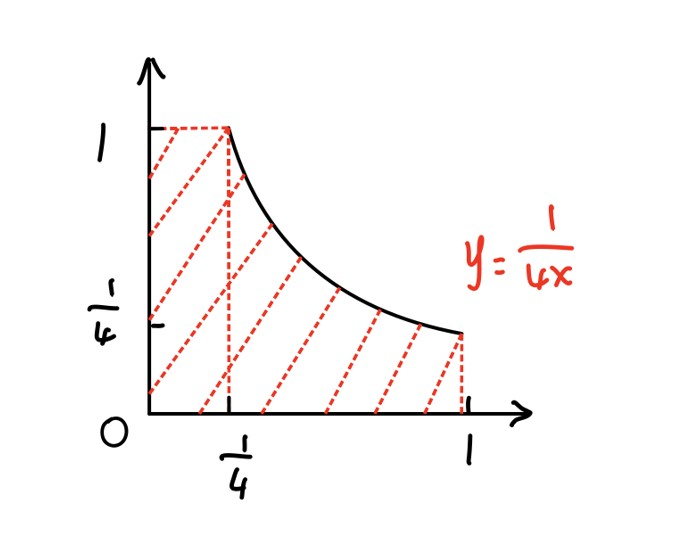
\includegraphics[width=0.7\linewidth]{几何概型.jpg}
	\caption{1.17附图}
\end{figure}
\section{1.18}
\begin{algorithm}
	\renewcommand{\algorithmicrequire}{\textbf{Input:}}
	\renewcommand{\algorithmicensure}{\textbf{Output:}}
	\caption{Calculate 1.18}
	\label{alg1}
	\begin{algorithmic}
		\STATE $N=0,RE=0$
		\WHILE{$N<=100000$}
		\STATE $a,b,c,d \gets random[0,1]$
		\IF {$a^2+\sin (b)+a*e^c\leq d$}
		\STATE $RE\gets RE+1$
		\ENDIF
		\STATE $N\gets N+1$
		\ENDWHILE
		\ENSURE $RE/100000$
	\end{algorithmic}
\end{algorithm}

$P=0.09408$
\section{1.19}
首先考虑将这9个元素作一个排列,共有9!种排列,但由于相同元素的排列没有区别,所以最后结果里应除以其对应阶乘的乘积.

即排列数S=$\frac{9!}{3!4!2!}=1260$
\section{1.20}
1.证明:$\binom{n}{r}+\binom{n}{r-1}=\frac{n!}{r!(n-r)!}+\frac{n!}{(r-1)!(n-r+1)!}\\
	=\frac{n!(n-r+1)}{r!(n-r+1)!}+\frac{n!r}{r!(n-r+1)!}\\
	=\frac{n!(n+1)}{r!(n-r+1)!}\\
	=\binom{n+1}{r}$

2.证明:$\binom{2n}{n}$可以理解为从两堆各含有n个元素的堆中共取出n个元素,那么可以从第一堆取出i个元素,从第二堆取出n-i个元素,即$\binom{2n}{n}=\sum_{i=0}^n\binom{n}{i}\binom{n}{n-i}$\\
又因为$\binom{n}{i}=\binom{n}{n-i}$.\\
故$\binom{2n}{n}=\sum_{i=0}^n\binom{n}{i}^2$

3.证明:该公式为上一个公示的变形,即两堆元素分别为m和n,不单为n,从中取出k个元素.

故易证$\binom{m+n}{k}=\sum_{i=0}^k\binom{n}{i}\binom{m}{k-i}$
\section{1.21}
1.无放回时共有$(m)_r$种排法.有放回时共有$m^r$种排法.
2.无放回时有$\binom{m}{r}$种组合,有放回时共有$\binom{r}{n+r-1}$种排法.

\section{1.22}
先求正整数解:对于不等式$x_1+x_2+...+x_k<=n$来说,其相当于将n个小球排成一列,除去第一个球之前的空隙,在其他的n个空隙中放置k个隔板,即有$\binom{n}{k}$种组合,即该不等式的正整数解的个数为$\binom{n}{k}$.

非负整数解:相当于求不等式$x_1+x_2+...+x_k<=n+k-1$的正整数解,共有$\binom{n+k-1}{k}$种不同的解.
\section{1.23}
正整数解:相当于用1.22求出的解减去对应方程的正整数解的个数,即正整数解共有$\binom{n}{k}-\binom{n-1}{k-1}=\frac{n!-k(n-1)}{k!(n-k)!}$个解.
非负整数解:相当于用1.22求出的解减去对应方程的正整数解的个数,即正整数解共有$\binom{n+k-1}{k}-\binom{n+k-1}{n}=\frac{(n-k)(n+k-1)!}{n!k!}$个解.
\section{1.24}
证明:\\
奠基:第二类stirling数的递推关系为$S(n,m)=mS(n,m-1)+S(n-1,m-1).$

已知S(0,0)=1,S(1,0)=1,由此可知S(n,0)=1.由S(1,1)=1,又S(n,1)=1.且每一个S(n,m)都可以通过递推式化为许多S(x,0)和S(y,1)的和.因此只需要证明递推式的关系正确.

$S(x,0)=1\times \sum_{i=0}^0(-1)^i\binom{0}{i}(0-i)^0=1.$

$S(y,1)=1\times \sum_{i=0}^1(-1)^i\binom{i}{i}(1-i)^1=1.$\\
归纳:设S(n-1,m)和S(n-1,m-1)都满足该式,则只需证明在该递推式下S(n,m)也满足该关系.

即需要证明$\frac{1}{k!}\sum_{i=0}^k(-1)^i\binom{k}{i}(k-i)^n=m\frac{1}{(k-1)!}\sum_{i=0}^{k-1}(-1)^i\binom{k-1}{i}(k-i-1)^n+\frac{1}{(k-1)!}\\\sum_{i=0}^{k-1}(-1)^i\binom{k-1}{i}(k-i-1)^{n-1}$

即证$\sum_{i=0}^k(-1)^k(k-1)!(k-i)^{n}=\sum_{i=0}^k!(k-i)^{n}+\sum_{i=0}^{k-1}(-1)^i(k-i)!(k-i)(k-i-1)^{n-1}$

化简后即证$(k-i)^{n-1}=k(k-i)^{n-1}+(m-i-1)^{n-1}$成立.然而我认为在化简的过程中我出了部分差错,导致该式无法继续证明.若能证明该式成立,则由归纳法知原式成立。




\end{document}